\section{引言(周盈坤)}
从2009年开始,云计算和云虚拟化方法取得了飞速的发展。在早期,市场选择了Amazon EC2这种针对云计算的low-level虚拟化方法\cite{jonas2019cloud},也即用户可以在云平台上,控制整个虚拟的软件栈。这与当时云计算的未来不明朗有着很大的关系。比起在云端系统上重新编写新的程序,早期的用户更希望在云平台上重新构建一个与本地机器上相同环境的系统,以简化将工作负载移植到云端的工作。但是这种初期市场的选择随着时间的推移,迎来了阵痛——要求开发人员自己管理虚拟机;而且随着业务系统架构的不断演进,系统中出现了越来越多的非业务基础技术需要支持,使得管理变得越来越复杂,最终导致开发人员需要掌握和关注的知识点越来越多。这种情况下,研发的门槛在上升,效率在下降。为了具体的说明这一点,文章\cite{jonas2019cloud}就详细列出了8个需要运维的方面:\textbf{1)}为了可用性的冗余,这样即使有机器出现故障也不会让整个系统宕机;\textbf{2)}异地容灾和备份机制;\textbf{3)}平衡负载和路由请求,已达到利用资源的高效性;\textbf{4)}系统的规模能够自动缩放以及时的响应复杂的变化;\textbf{5)}检测确保服务仍在正常运行;\textbf{6)}记录日志,为了调试和性能调优之需;\textbf{7)}系统升级,包括安全补丁;\textbf{8)}将服务迁移到新的变为可用的实例上。

上述的每一个方面都不是省油的灯,需要投入大量人力物力资本才能解决,对于小规模的公司而言,系统全栈式显然不合理。而且这种全栈式的管理对于简单的应用也是不合理的。比如一个只是执行将手机端的图片上传到云端的应用,逻辑代码可能只是几十行JavaScript代码,可是要让这个代码运行起来,却需要投入大成本设置适当的服务器环境。杀鸡焉用宰牛刀!\textbf{让业务系统研发更专注于本身的业务逻辑,这样的诉求在云计算快速发展的同时也愈发强烈。}于是乎,Amazon在2015年推出了AWS Lambda来提供cloud functions(云函数)这样的Serverless Computing服务(serverless cloud体系结构如图\ref{figs:architecture1}所示)。
\begin{figure}[!htbp]
	\centering
	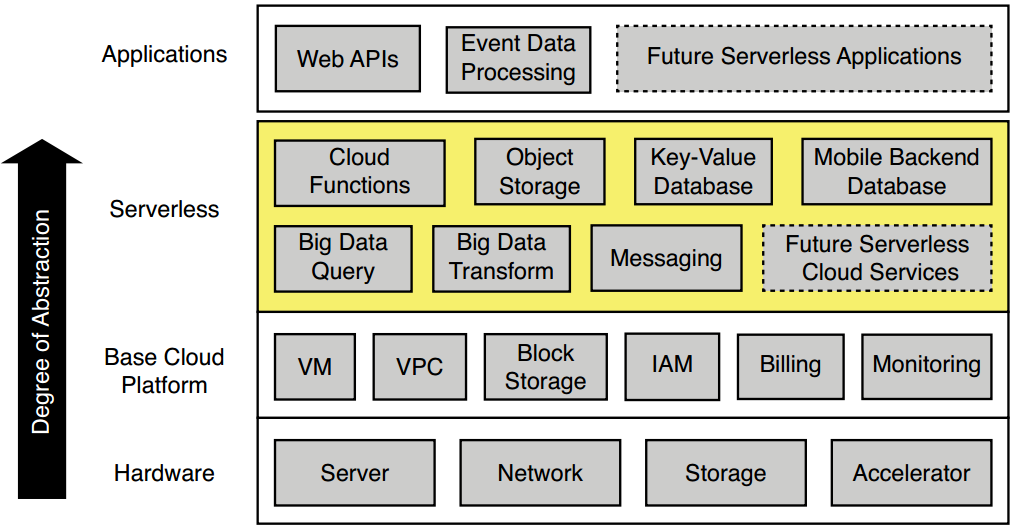
\includegraphics[width=0.8\linewidth]{figs/architecture}
	\caption{Serverless cloud体系结构。serverless层位于应用层和基础云平台之间,简化了云编程。Cloud Functions(例如FaaS)提供了通用的计算并且实现在了专门的BaaS生态(有对象存储,数据库和讯息的服务)中。更具体的,一个在AWS生态中的Serverless应用除了使用Lambda来运行函数外,可能会配套的使用S3(对象存储)和DynamoDB(键值数据库);一个在Google's cloud上的使用Cloud Functions可能配套有Cloud Firestore(移动后端数据库)和Cloud Pub/Sub(讯息)。Serverless还会包含特定的大数据服务如AWS Athena和Google BigQuery,和Google Cloud DataFlow和AWS Glue(大数据传输)。另外在基础平云台上,由供应商提供的有VM,私有网络(VPC,private networks),虚拟化的块存储,用于身份认证的IAM(Identity and Access Management),同时还有后台的计费和事实监测服务。(\cite{jonas2019cloud}图1)}
	\label{figs:architecture1}
\end{figure}
用户只需要编写并上传代码,声明触发事件;Serverless服务供应商就会负责实例出函数执行所需的系统环境来执行该函数,涵盖了实例选择、自动缩放、代码与数据部署、容错、日志、安全补丁和版本更新等脏活累活。

自此,Serverless computing成为了近几年来云计算领域最为火热的概念之一。根据谷歌查询请求的搜索关键词趋势显示,其热度甚至可以和之前如日中天的MapReduce概念的巅峰时期相媲美,如图\ref{figs:trend}所示。
\begin{figure}[!htbp]
	\centering
	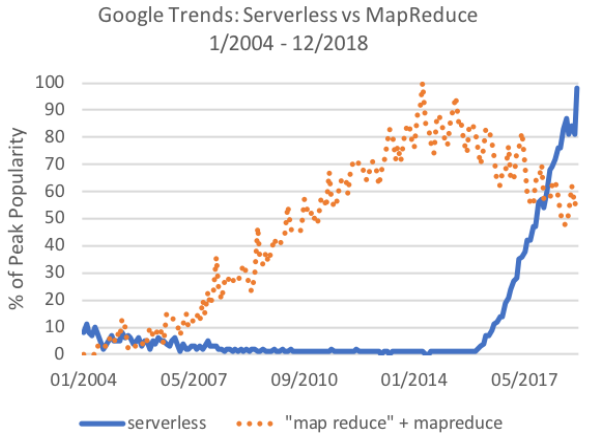
\includegraphics[width=0.5\linewidth]{figs/trend}
	\caption{$ 2014\sim2018 $年谷歌搜索关键词``Serverless''和``MapReduce''的趋势对比。(\cite{hellerstein2018serverless}图1)}
	\label{figs:trend}
\end{figure}
但事实上Serverless computing是一个非常模糊的概念,并没有一个清晰的定义,每个Serverless云平台的供应商(Amazon、Google、Microsoft)都有自己的一套解读并以营销的手段推广之。但基本的思路都是:应用开发人员只需要向云平台上传自己的代码(当今的FaaS产品都支持多种语言,例如Python、Java、JavaScript、Go)完成注册函数;声明触发每个功能的事件;接着FaaS架构会监视这些触发事件;由云平台的供应商来管理资源的分配与调度,为用户定义的函数分配运行时(runtime),按需自动缩放(autoscaling)函数执行的运算资源,并将结果持久化\cite{hellerstein2018serverless};而用户仅需要按照函数实际执行时间付费,也即pay-as-you go模式。这样,程序开发者不需关心服务器的配置和运行,可以看做是``Serverless''概念最直观的理解。以AWS Lambda为例,Serverless模式如图\ref{figs:flow}所示。
\begin{figure}[!htbp]
	\centering
	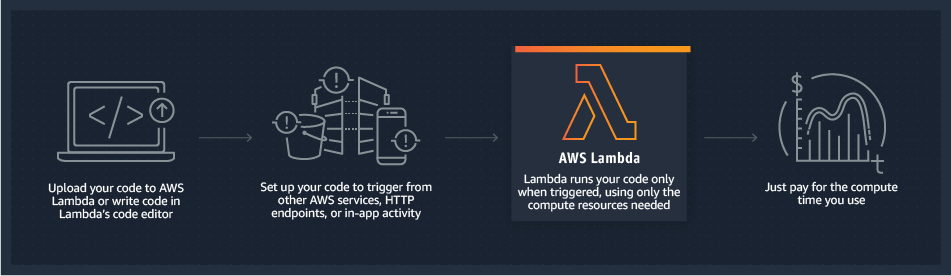
\includegraphics[width=0.7\linewidth]{figs/flow}
	\caption{AWS Lambda运作模式\cite{lambda}。}
	\label{figs:flow}
\end{figure}

虽然我们不计较Serverless computing的精确概念,但是仍然有必要厘清楚两对容易混淆的技术概念之间的关系。

\textbf{Serverless computing和Lambda/FaaS(Function as a Service)的关系}。Cloud functions属于FaaS范式;而FaaS被视为是Serverless computing的核心理念。但是FaaS本身提供不了什么价值,函数执行短暂而且互相隔离;除了触发以及自动扩展函数执行的机制外,在FaaS上构建应用程序还需要在持久和临时存储中进行数据管理\cite{hellerstein2018serverless}。所以虽然Severless的概念是由Lambda/FaaS兴起的,但是两者并不等同。Serverless不仅仅是FaaS,还需要加上由供应商提供的各式各样多租户自动缩放服务的``标准库''支持;对于AWS来说,这包括S3(大对象存储)、DynamoDB(键值存储)、SQS(排队服务)、SNS(通知服务)等\cite{hellerstein2018serverless}。换言之,云平台为了迎合特定应用的需求,还提供了以BaaS(Backend as a Service,如Serverless数据库、对象存储和大数据处理服务等形式存在的Serverless框架。一种简单的理解是:Serverless Computing = FaaS$ + $BaaS\cite{jonas2019cloud}.

\textbf{Serverless computing和Kubernetes的关系}。Kubernetes作为一种``容器编排''技术是用来部署微服务(microservices)的\cite{jonas2019cloud}。微服务和Serverless computing又有着千丝万缕的关联,但这里我们就不展开讨论了。Kubernetes本质上是一种简化的Serverful computing管理技术。由于多年来Google内部的开发和使用,它得以快速发展。虽然脱胎于Serverful computing,但是Kubernetes可以提供短期的计算环境,和Serverless理念一拍即合,并在硬件资源、执行时间和网络通信方面有更少的限制。托管的Kubernetes产品有Google Kubernetes Engine(GKE)和AWS Elastic Kubernetes Service(EKS),另外微软的Azure Serverless云系统的实现也是基于Kubernetes。但是托管式的Kubernetes服务和Serverless服务之间有一个关键区别:\textbf{计费模型}——前者按照分配的资源收费,而后者按照函数执行时间,也即真实使用的资源收费\cite{jonas2019cloud}。由此可见,虽说Kubernetes不是为了Serverless专门设计的,但是工业界还是很会普遍的复用Kubernetes,通过在其上进行封装使得Serverful的逻辑对上层用户不可见来实现Serverless computing。

总结一下,Serverless计算和传统的与之对立的Serverful计算有四个关键的不同之处:
\begin{enumerate}
	\item 用户执行代码不需要管理资源分配。而且这些代码大多功能单一,无状态。
	\item Serverless平台责任方根据实际计算的需要,快速地对资源进行自动缩放(autoscaling)。
	\item 计算与存储解耦合。数据存储由另外的云服务来提供服务。因此两者的分配和价位彼此独立。
	\item 以使用的资源付费(如执行时长)而不是分配的资源(如分配的VM的大小和数量)。
\end{enumerate}

本报告后面章节的安排如下:
\begin{itemize}
	\item \textbf{周盈坤}\ \ 章节\ref{sec:lambda}初步介绍Amazon AWS Lambda云平台的使用和早期实现;章节\ref{sec:berkeley}解读伯克利分校的学者对于Serverless computing的见解,围绕着两篇最近一两年的论文展开;章节\ref{sec:Firecracker}对Lambda Serverless平台做更深入的调研,以介绍开源项目Firecracker为主;
	\item \textbf{汪钇丞}\ \ 章节\ref{sec:microsoft}讲解了Microsoft在Serverless computing上的具体实现Azure云平台的设计与架构。
	\item \textbf{胡登杭}\ \ 章节\ref{sec:serverless_DB}更为深入地调研了Azure云平台函数的持久化和存储;并以Azure Data Lake Store为主体介绍了Serverless DB的设计与架构。
	\item \textbf{汪润川}\ \ 章节\ref{sec:implementation}调研了论文\cite{mcgrath2017serverless}介绍的自实现的一个简单的Serverless平台原型;章节\ref{sec:google_cloud}阐述了Knative与Google Cloud Run的具体设计与架构。可贵的是,在章节\ref{sec:google_cloud}还给出了在Google云平台上具体的实践操作!
	\item \textbf{刘力玮}\ \ 章节\ref{sec:azure_use}详述了在Microsoft Azure云平台程序开发的流程;章节\ref{sec:google_use}详述了在Google Cloud Functions云平台上程序开发的流程。
\end{itemize}
总的来说,我们研究小组对Serverless computing调研的范围涵盖了该领域的三巨头:Amazon、Microsoft和Google推出的Serverless computing产品。不仅以程序员的角度详细介绍了在这些Serverless云平台上,应用的开发流程与编程界面;而且以系统架构师的角度,深入地考察了这些平台的工作原理,以及系统对Serverless computing function支持的具体设计实现架构。同时还结合穿插了近期论文的阅读,使得整个报告更加详实。

\section{Amazon AWS Lambda初探(周盈坤)}\label{sec:lambda}
Amazon的AWS Lambda是第一个提出Serverless服务的云平台。但这个结论并不是没有争议的。一些人可能会指出上世纪90年代流行的共享web主机环境提供了许多Serverless computing范畴的功能;例如它们也有无状态的编程模型、多租户模式、对可变需求的强行响应和一套标准化的函数调用API、公共网关借口(CGI)、甚至允许直接部署用Perl或PHP等高级语言编写的代码\cite{jonas2019cloud}。而作为Amazon EC2的老对手,Google最初的App Engine也允许开发者直接部署代码,同时大部分的操作交由云平台来完成。但是App Engine模式在Severless正式流行的这几年之前,基本上不被市场所接纳,惨败于EC2模式。那么Lambda既然带火了Serverless,就一定有其过人之处。它与之前产品的最大不同指出在于提供了真正能够大规模运用的自动缩扩容能力,跟踪应用的负载,快速响应资源需求。如在没有需求的情况下能将资源一直缩减为零;并以一种更加细粒度的方式管理,如最小时长单位为100ms的按时计费服务。
\subsection{The use cases}
百闻不如一见,我们首先来见识几个使用Lambda函数的实际用例。下面给出6个Severless computing的使用案例。为了论述的完整性,这里简单阐述一下用例中使用的backend服务的作用(参考\href{https://aws.amazon.com/serverless/}{AWS Serverless}官网)。
\textbf{Amazon S3(Simple Store Service):}提供安全、持久且高扩展性的对象存储服务,同时易于使用,具有简单的Web服务端口,用于在Web上的任何位置存储和检索任意数量的数据;
\textbf{Amazon Kinesis:}是一种AWS上流式处理数据的平台,可以帮助开发者轻松加载和分析流数据,另外还能让开发者根据具体需求来构建自定义流数据应用程序;
\textbf{Amazon DynamoDB:}快速灵活的NoSQL服务,适合所有需要一致性且延迟低于10毫秒的任意规模的应用程序;
\textbf{Amazon Redshift:}是种快速且完全托管的数据仓库服务,让开发者可以使用标准SQL和现有的商业智能工具经济高效地分析用户的所有数据,提供优质的数据仓库解决方案;
\textbf{Amazon API Gateway:}提供完全API托管服务,可以帮助开发者轻松创建、发布、维护、监控和保护任意规模的API,同时可以帮助开发者处理成千上万个并发API调用和流量管理、授权、访问控制、监测以及API版本管理;
\textbf{Amazon SNS:}一种完全托管的发布/订阅消息收发服务,可以轻松分离和扩展微服务、分布式系统和Serverless应用程序。
\begin{enumerate}
	\item 实时文件处理应用。如图\ref{figs:eg3}使用S3来触发AWS Lambda,将Lambda函数对上次的拍摄的照片进行根据桌面手机的不同屏幕大小实时调整图片大小。Lambda函数类似的功能还有实时创建缩略图、转换视频代码、建立文件索引、处理日志、验证内容以及聚合和筛选数据。
	\item 物联网IoT后端应用。如图\ref{figs:eg6}将传感器的数据发送到Kinesis上,接着由Kinesis触发AWS Lambda;Lambda根据规则自动进行订单的组装。
	\item 实时数据流处理应用。如图\ref{figs:eg4}使用Kinesis实时地将社交媒体流数据加载进来,触发AWS Lambda;Lambda运行函数产生哈希标签趋势数据(hashtag trend data);这些数据会存入DynamoDB中,用来提供商业用户对这些社交媒体趋势数据的及时查询。类似的功能还有通过实时流数据跟踪应用程序活动、整理数据、生成指标、筛选日志、建立索引、分析社交媒体以及遥测和计量IoT设备数据。
	\item 数据仓库中的大数据分析应用。如图\ref{figs:eg5}展示了电子商务公司普遍存在的一个应用场景——对用户的购物行为进行分析。线上的订单数据会被存入DynamoDB中;AWS Lambda针对DynamoDB表中每个数据更改执行数据验证、筛选、排序或者其他转换(ETL, database Extract, Transform, and Load);接着将转化后的数据加载到RedShift数据仓库中;最后从数据中自动产生分析。
	\item Web应用程序。这是一类非常流行的应用,用到了如图\ref{figs:eg1}所示的同步调用的模式,其中关键的一点是使用API Gateway。对于这个搜索当地天气信息的App来说,网页前端的代码会从S3中经由用户点击这个时间传送到API Gateway;接着触发AWS Lambda运行代码从DynamoDB中获得天气的信息并且返回数据给用户。
	\item 移动后端应用。如图\ref{figs:eg2}展示了媒体社交平台普遍存在的一个应用场景——用户发布了自己的更新状态,平台App通过API Gateway触发AWS Lambda;Lambda函数会查看用户的朋友列表并且初始化状态更新的通告;接着状态更新通告就会通过SNS服务推送给用户的朋友;这些朋友们就能在自己的移动端接收到状态更新通告了。
\end{enumerate}
%TODO: https://aws.amazon.com/lambda/
\begin{figure}[!htbp]
	\begin{subfigure}[b]{0.49\linewidth}
		\centering
		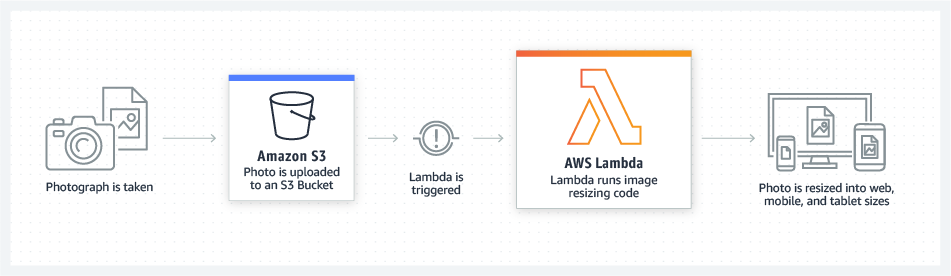
\includegraphics[width=\linewidth]{figs/eg3}
		\caption{}
		\label{figs:eg3}
	\end{subfigure}
	\begin{subfigure}[b]{0.49\linewidth}
		\centering
		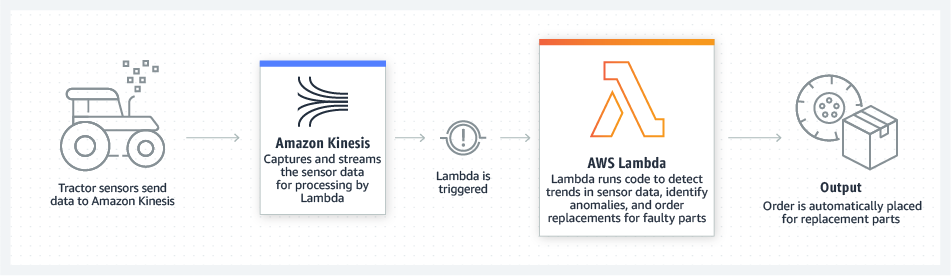
\includegraphics[width=\linewidth]{figs/eg6}
		\caption{}
		\label{figs:eg6}
	\end{subfigure}
	\begin{subfigure}[b]{\linewidth}
		\centering
		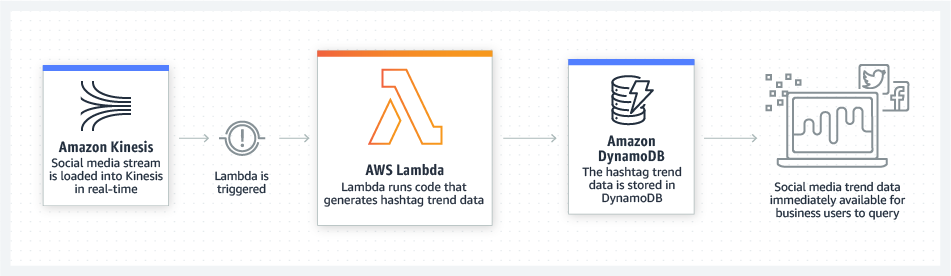
\includegraphics[width=0.8\linewidth]{figs/eg4}
		\caption{}
		\label{figs:eg4}
	\end{subfigure}
	\begin{subfigure}[b]{\linewidth}
		\centering
		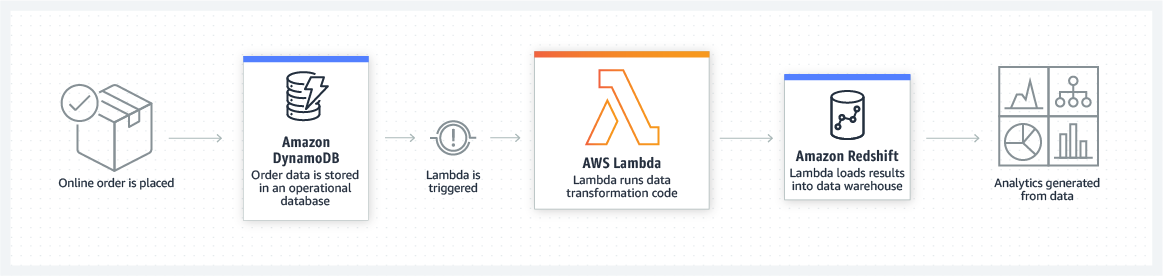
\includegraphics[width=0.8\linewidth]{figs/eg5}
		\caption{}
		\label{figs:eg5}
	\end{subfigure}
	\begin{subfigure}[b]{\linewidth}
		\centering
		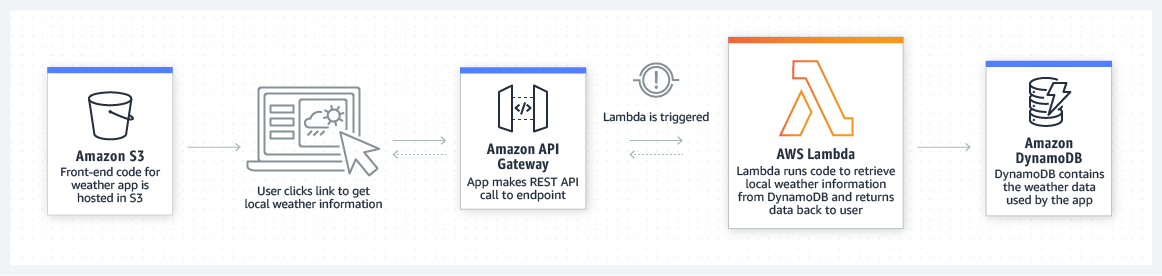
\includegraphics[width=0.8\linewidth]{figs/eg1}
		\caption{}
		\label{figs:eg1}
	\end{subfigure}
	\begin{subfigure}[b]{\linewidth}
	\centering
	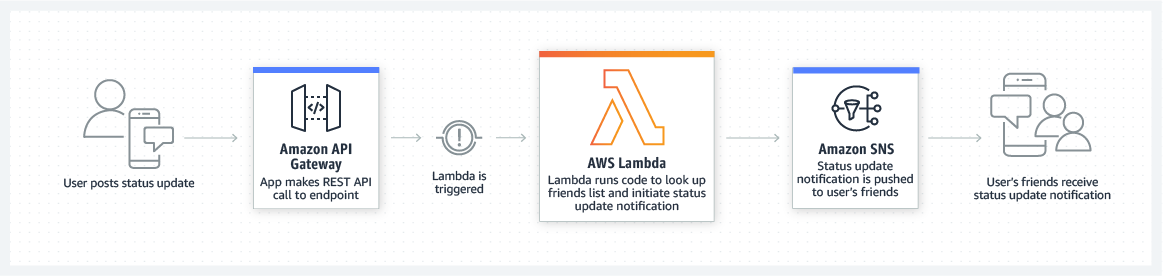
\includegraphics[width=0.8\linewidth]{figs/eg2}
	\caption{}
	\label{figs:eg2}
	\end{subfigure}
	\caption{(a) 实时文件处理应用。(b) 物联网IoT后端应用。(c) 实时数据流处理应用。(d) 数据仓库中的大数据分析应用。(e) Web应用程序。(f) 移动后端应用。\cite{lambda}}
	\label{}
\end{figure}
表\ref{tab:usage}中展示的是\cite{serverless}在2018年统计的6大Serverless computing使用最多的应用场景,和上述的6个实际用例相呼应。
\begin{table}[!htbp]
	\caption{Popularity of serverless computing use cases according to a 2018 survey\cite{serverless}.}
	\label{tab:usage}
	\centering
	\footnotesize% fontsize
	\setlength{\tabcolsep}{4pt}% column separation
	\renewcommand{\arraystretch}{1.2}%row space 
	\begin{tabular}{ll}
		\hline
		占比 & 用例\\%inserts table 
		\hline
		32\%   & Web and API serving. 如例子\ref{figs:eg1}和\ref{figs:eg2}所示。\\
		21\%   & Data Processing, e.g., batch ETL (database Extract, Transform, and Load). 如例子\ref{figs:eg4}和\ref{figs:eg5}所示。\\
		17\%   & Integrating 3rd Party Services. \\
		16\%   & Internal tooling. 如例子\ref{figs:eg3}所示。\\
		8\%    & Chat bots e.g., Alexa Skills (SDK for Alexa AI Assistant). \\
		6\%    & Internet of Things. 如例子\ref{figs:eg6}所示。\\
		\hline
	\end{tabular}
\end{table}

从具体的实际用例中抽象出来,Lambda函数有三种不同形式的调用方式。分别是同步(Synchronous)调用、异步(Asynchronous)调用和基于轮询(Poll-Based)调用,如图\ref{figs:invoke}所示。\\
同步调用是最直接的一种方式,由API Gateway来调用,如例子\ref{figs:eg1}和\ref{figs:eg2}所示。反映在命令行中为:
\begin{lstlisting}[language=bash]
aws lambda invoke —function-name MyLambdaFunction —invocation-type RequestResponse —payload  “[JSON string here]”
\end{lstlisting}
异步调用是事件驱动的。Amazon的S3和SNS等服务都可以产生事件来调用Lambda函数,如例子\ref{figs:eg3}和\ref{figs:eg5}所示。反映在命令行中为:
\begin{lstlisting}[language=bash]
aws lambda invoke —function-name MyLambdaFunction —invocation-type Event —payload  “[JSON string here]”
\end{lstlisting}
基于轮询调用主要是为了实时性的服务而设计的,比如加载流数据的Kinesis和产生流数据的DynamoDB Streams,如例子\ref{figs:eg6}和\ref{figs:eg4}所示。
\begin{figure}[!htbp]
	\centering
	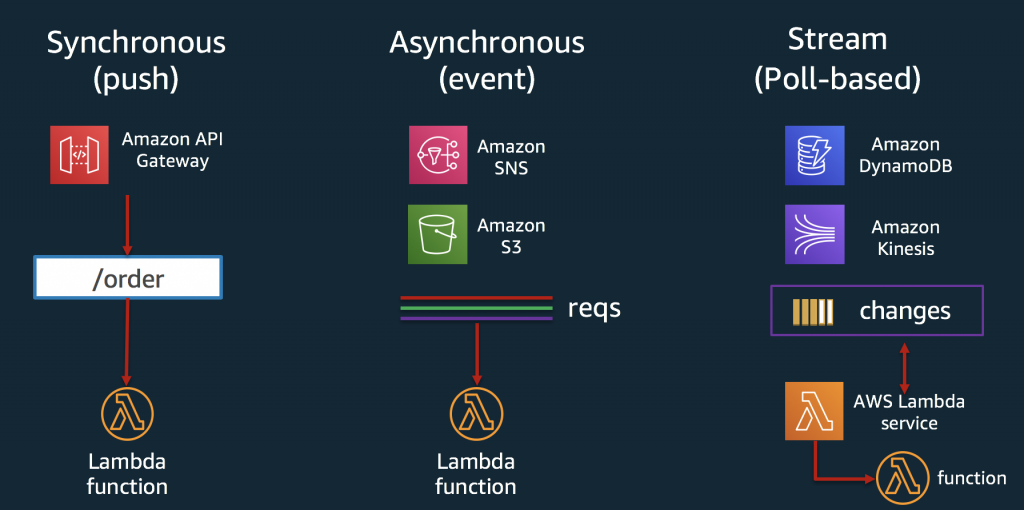
\includegraphics[width=\linewidth]{figs/invoke}
	\caption{三种调用Lambda函数的方式\cite{invoke}。}
	\label{figs:invoke}
\end{figure}

所以从AWS Lambda上,我们可以看到当下的Serverless computing相较之前的产品要成熟得多,得益于背后Amazon强大完整的生态支持(BaaS的思想),得益于更好的自动缩扩容、更安全的隔离性和更灵活的云平台。Serverless computing大多采用多租户共享硬件的模式,所以依赖于高性能和隔离安全性。VM或容器提供的隔离是当前cloud function下多租户的事实上的标准。但是因为VM或者容器配置(冷启动)需要很长的时间,为了缩短这个时间,Serverless computing供应商使用复杂的技术来加快函数运行环境的创建。AWS Lambda中使用的方法是维护一个VM实例``热池'',和一个之前执行过的函数实例的``活跃池''以快速响应未来可能到来的调用\cite{jonas2019cloud}。资源的生命周期管理和多租户下的bin packing是Serverless computing中提高资源利用率以及性能的核心技术。所以近几年来的一些工作旨在通过利用Unikernel、Firecracker、gVisor等技术来减少多租户隔离所带来的开销。

\subsection{Serverless computing architecture之AWS Lambda implementation}
\begin{figure}[!htbp]
	\begin{subfigure}[b]{0.49\linewidth}
		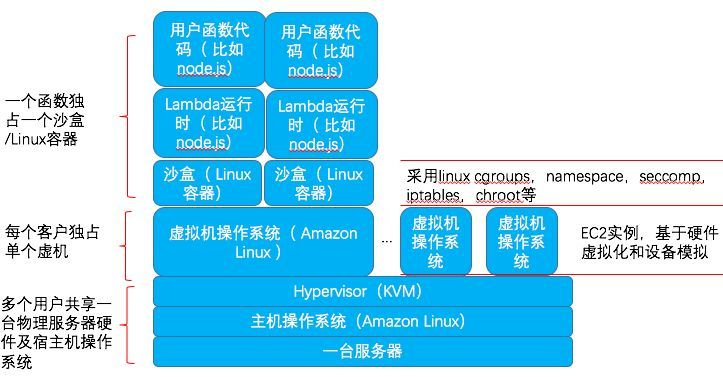
\includegraphics[width=\linewidth,height=0.21\textheight]{figs/arch}
		\caption{}	
	\end{subfigure}
	\begin{subfigure}[b]{0.49\linewidth}
		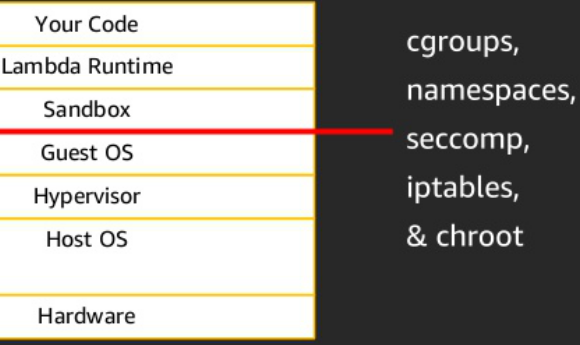
\includegraphics[width=\linewidth]{figs/stack_0}
		\caption{}
		\label{figs:stack_0}
	\end{subfigure}
	\caption{(a) AWS Lambda Serverless云平台早期架构\cite{luodi}。(b) AWS Lambda Serverless云平台软硬件栈\cite{reinvent}。}
	\label{figs:arch}
\end{figure}

在Serverless computing的架构中,还需要考虑的因素的因素有负载平衡、故障处理等。下面我们来介绍Amazon早期对Serverless computing的实现。Lambda早期是将用户函数运行在独占的EC2虚拟机中的Linux容器上的。其架构和软硬件栈如图\ref{figs:arch}所示。Linux容器采用Linux控制组(cgroups)和命名空间(namespace)。其中,cgroups定义进程的使用资源(CPU、内存、网络等);namespace定了一个进程的访问权限(uid, gid, pid, mount, filesystem等)。除了cgroups和namespace,Linux容器还会使用到seccomp技术。seccomp是内核防火墙,限制一个进程对内核系统调用systemcall的访问权限,因此能够在应用程序和内核之间提供更好的隔离。但是它们要求用户创建预定义的系统调用白名单。然而在实际中,很难事先罗列出应用程序所需要的所有系统调用。因此容器之上还需要用沙盒(sandbox)来加固隔离安全性。

\begin{figure}[!htbp]
	\centering
	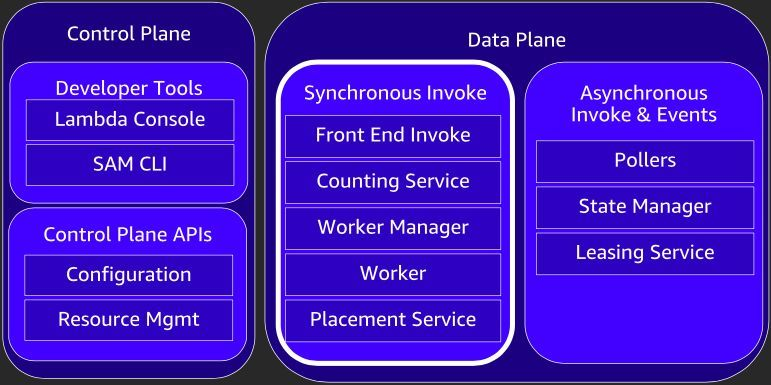
\includegraphics[width=0.6\linewidth]{figs/internal}
	\caption{AWS Lambda Serverless云平台技术架构\cite{reinvent}。}
	\label{figs:block}
\end{figure}
\begin{figure}[!htbp]
	\centering
	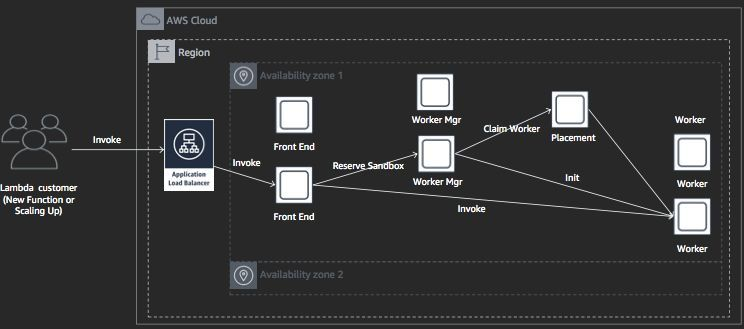
\includegraphics[width=0.8\linewidth]{figs/worker}
	\caption{用户编写的函数在AWS Lambda中运行的基本流程概念图\cite{reinvent}。}
	\label{figs:worker}
\end{figure}
如图\ref{figs:block}展示了Lambda的技术架构。
这里我们将目光聚焦在中间白色粗边框起来的部分,其中:Front End Invoke能够编排同步调用也能编排异步调用;Counting Service提供了一个用户并发的域范围视角来强制设置限额;Worker Manager追踪容器空闲和忙碌的状态,并且为新来的函数调用请求调度可用的容器;Worker为用户代码提供一个安全的执行环境;Placement Service将沙盒放置在workers上,在不影响用户体验或者冷路径延迟(cold-path latency)的前提下,最大化packing的密度。
具体地,或者更为直观的理解,在早期一个worker就是一个EC2实例,其操作系统为Amazon Linux。
图\ref{figs:worker}是worker被创建以及函数被调度到worker中的基本流程。
其中,Worker manage负责worker的创建和管理,Placement负责将用户的函数调度到某个或某些worker上运行。流程为:用户请求通过ALB(Application Load Balancer)转发给Front End;接着Front End发送请求至Worker Manager;Worker Manager初始化Worker;Worker准备函数沙盒执行环境;Worker启动后将状态原路返回给Front End;最后交由Front End触发函数执行。

用AWS Lambda软硬件栈的视角来看,如图\ref{figs:stack}所示。用户函数运行在Lambda Runtime中;再下面是沙盒;沙盒的下边界(见图\ref{figs:stack_0})使用了cgroups, namespaces, seccomp, iptables和chroot等结构以实现操作系统层级上的虚拟化;再往下两层是实现安全隔离的关键——虚拟化技术与设备模拟。
\begin{figure}[!htbp]
	\begin{subfigure}[b]{0.49\linewidth}
		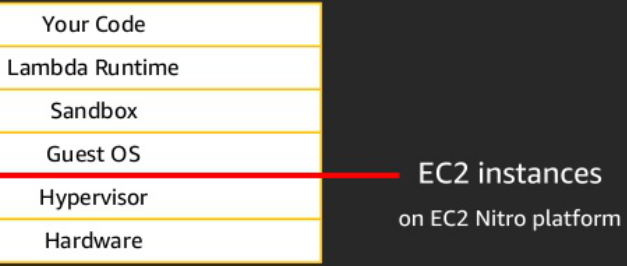
\includegraphics[width=\linewidth]{figs/stack}
		\caption{}
		\label{figs:stack}	
	\end{subfigure}
	\begin{subfigure}[b]{0.49\linewidth}
		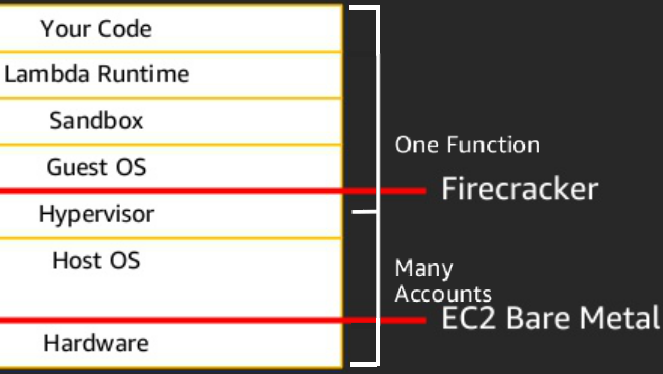
\includegraphics[width=\linewidth]{figs/stack_2}
		\caption{}
		\label{figs:stack_2}
	\end{subfigure}
	\caption{(a) EC2在软硬件栈中的位置。(b) Firecracker在软硬件栈中的位置。\cite{reinvent}}
\end{figure}
早期的Lambda服务始于EC2实例上构建worker,好处有:1)安全边界清晰;2)快速构建系统并上限业务。但是Amazon后来意识到,基于EC2实例的Lambda存在着明显的缺陷:
\begin{itemize}
	\item 浪费资源:用户一个简单的测试函数也会占用一个EC2虚机。
	\item 启动速度:EC2虚机的创建时间很长。
	\item 管理复杂:需要管理复杂的资源和安全模式。
\end{itemize}
并不适合今天Serverless computing的需求——资源利用率高、启动快、有更好的扩展性同时管理便捷。为了达到以上三点,并且不以损失性能为代价,Amazon决定对早期的Lambda进行改进,在此过程中开发了Firecracker微虚机,如图\ref{figs:stack_2}所示。更深入的介绍参见章节\ref{sec:Firecracker}。接来下的章节\ref{sec:berkeley}我们先来看看来自伯克利分校的学者对于Serverless computing的见解。

\section{Serverless Computing之Berkeley Views(周盈坤)}\label{sec:berkeley}
2018年年底和2019年年初,时隔两个月的时间,加州大学伯克利分校的学者们(出自同一个实验室)发了两篇近几年来在Serverless Computing领域颇有影响力的文章\cite{hellerstein2018serverless,jonas2019cloud}。将这两篇论文对比起来看可以发现:一个唱红脸一个唱白脸,非常有意思。前者\cite{hellerstein2018serverless}唱白脸,负责泼冷水,砸Serverless Computing的场子,犀利的指出第一代Serverless computing的局限性和关键缺陷;后者\cite{jonas2019cloud}唱红脸,负责回顾,总结和展望Serverless Computing,并乐观的认为:实现和完善是一步一步来的,各种工程上的挑战也都是暂时的,Serverless Computing有着光明的未来。我们依次来解读这两篇文章。

\subsection{Serverless Computing: One Step Forward, Two Steps Back}
文章\cite{hellerstein2018serverless}试图提醒人们在跟风追求潮流的时候,应该回归理性,用批判性的思维来审视Serverless computing。这篇文章为了避免泛泛而谈,选择了AWS的FaaS框架的Lambda作为明确的讨论主体。

首先,按照函数的调用交互可以将Serverless use cases划分为3个类别\cite{hellerstein2018serverless}:
\begin{enumerate}
	\item 尴尬的并行函数。每个函数都是独立的任务,不需要和其他函数交互和相互通信。而且要求这些任务能够在短时间内比如几分钟完成。这类应用能够直接利用Lambda自动缩放的特性来按需向上或向下扩展。
	\item 编排函数。利用Serverless函数来完成简单的服务调用编排。例如在Lambda上实现查询服务应用。具体的查询以及数据处理是由Amazon提供Athena和S3的云服务来完成的,Serverless函数在这里值起到一个统筹指挥的作用。
	\item 函数组合。应用是由函数的集合组成的,这些函数串在一起,上一个函数的输出是下一个函数的输入。这些函数通常要操作状态,所以往往和排队系统(比如SQS)或者对象存储(比如S3)
\end{enumerate}
总的来说,Serverless以及目前的FaaS方案对第一中类别的应用场景更具有吸引力,也即简单的、独立的任务,并且相互之间没有通信。而use cases中如果包含了有状态的任务,则就有令人无法接受的高延迟——云供应商宣传的10分钟长周转时间。

下面回到正题:对标题\textit{Serverless Computing: One Step Forward, Two Steps Back}的阐述。自然地,分成了两个方面:
\begin{enumerate}
	\item \textbf{One Step Forward的观点}\begin{quote}
		By providing autoscaling, today's FaaS offerings take a big step forward for cloud programming, offering a pratically manageable, seemingly unlimited compute platform.\cite{hellerstein2018serverless}
	\end{quote}
	Serverless使得能够弹性地、按照需求地使用云资源,是一大进步。
	\item \textbf{Two Steps Back的观点}\begin{quote}
		First, they painfully ignore the importance of efficient data processing. Second, they stymie the development of distributed systems.\cite{hellerstein2018serverless}
	\end{quote}
	两个退步的地方:首先因为每个函数是彼此隔离运行的,而且是无状态的。所以它们之间的交互是通过持久或临时的存储、事件驱动来完成的。这样导致了完成交互的时间比传统架构慢了很多;其次通常分布式系统会依赖如Leader选举、数据一致性和事务提交的技术机制,而这些在目前的FaaS平台上是很难去实现的。
\end{enumerate}
比起One Step Forward进步方面,从篇幅上来看,作者显然是想强调Two Steps Back退步方面。在进步方面,文章花费的笔墨很少,只提到各大供应商都宣传的三大关键特性:1)无限的数据存储,无限的分布式计算能力,以及按照使用的资源付费,而不是以所需要资源的峰值持续付费。接下来的大段篇幅都是在揭Serverless computing的短处。首先是Severless的局限性,以AWS Lambda为例,陈列了如下四点\cite{hellerstein2018serverless}:
\begin{enumerate}
	\item \textbf{受限的存活时间}\ \ 函数调用如果超过15分钟,会被Lambda停止。虽说Lambda可能会将函数的状态缓存入当前运行的主VM上,来支持热启动。但是没有机制能够保证下次执行该函数是在同一个VM上。
	\item \textbf{I/O瓶颈}\ \ 目前FaaS通过网络借口的方式来连接云服务,尤其是共享存储。网络限制了I/O吞吐量。最近的研究表明单个Lambda函数的平均网络带宽是538Mbps,当然了,Google和Azure也是半斤八两,比单个现代SSD慢了一个数量级。更糟糕的是,在一个VM上往往有多个函数共享带宽——假设有20个,那么每个函数的平均带宽只有可怜的28.7Mbps.
	\item \textbf{通过低速存储进行通信}\ \ Lambda函数在运行时不能以任何方式直接进行网络寻址。结果是,两个Lambda函数只能通过自动缩放的中间服务(比如S3)进行通信;这意味着像S3存储系统比点对点的网络速度更慢,成本更高。跨客户端调用维护状态需要将状态写入慢速存储,并在每次后续调用时将其读出。而这个读写状态的延迟高的可怕。例如,在处理客户端请求时,每个函数被分配到流程中的一个子任务。每个子任务都应该知道当前请求的上下文,也就需要保存会话状态。但是Serverless的无状态特性使得每个子任务的会话信息不能直接共享,需要像保存到慢速的存储服务如S3中,然后下游的子任务在从S3中获取上下文,接着执行。
	\item \textbf{无专用硬件}\ \ FaaS/Lambda目前只支持设置CPU超线程的时间片和内存使用量,而对GPU等专用硬件的支持不够——没有API或其他机制来访问这些专用加速硬件。
\end{enumerate}

上述的局限性会直接推导出如下的问题\cite{hellerstein2018serverless}:
\begin{enumerate}
	\item \textbf{FaaS是Data-shipping架构}\ \ 这可能是FaaS平台和其APIs最大的架构缺陷。Serverless函数运行在隔离的VM上,与数据分离。此外,Serverless函数是短暂存在的其不可寻址的,因此它们在内部缓存状态以服务重复请求的能力是有限的。所以FaaS通常是``将数据传送到代码(shipping data to code)'',而不是``将代码传送到数据(sihpping code to data)''。但是存储器层次结构的实际情况——跨越各种存储层和网络延迟——由于延迟、带宽和成本的原因,使得data-shipping是一个糟糕的设计。
	\item \textbf{FaaS阻碍了分布式计算的发展}\ \ 由于Serverless函数没有网络可寻址性,因此只有通过缓慢而昂贵的存储传递数据,两个函数才能以Serverless的方式系统工作。这阻碍了基于细粒度通信协议如leader选举、成员资格、数据一致性和数据提交。很多分布式和并行应用程序——尤其是科学计算——也依赖于细粒度的通信。尽管另一种看法是FaaS鼓励基于全局状态的新的事件驱动的分布式编程模型。但是事件处理仍然需要将全局状态的部分从慢速存储传递到Serverless函数。同时,当前的Serverless存储在副本之间提供了弱一致性。
	\item \textbf{FaaS阻碍了有硬件加速的软件创新}\ \ 当前的FaaS产品都运行在统一且相当平凡的VM平台上,没有提供GPU等用户自定义的硬件加速的软件执行机制。但是可喜的是,中国的企业如华为已经提供了支持GPU加速的Serverless云平台,可以参见网址\url{https://www.huaweicloud.com/product/cci.html}. 此外FaaS平台也无法支持内存数据库系统——最大的Lambda实例也只被允许最大3GB的RAM。缺乏对这些硬件的访问以及适当的定价模型,显著限制了FaaS产品作为软件创新平台的效用。
	\item \textbf{FaaS不鼓励开源服务的创新}\ \ 流行的开源软件基本上都是有状态的,所以不能在当前Serverless架构中大规模运行。特别是近年来快速增长和成熟的领域——开源数据库系统,将无法在当前的FaaS平台上进行构建。并且,当前Serverless基础架构有意或无意地将用户锁定在平台供应商提供的服务器上。
\end{enumerate}

为了真实的评估这些问题的严重性,文章\cite{hellerstein2018serverless}研究了三个从大数据到分布式计算设置的实例,分别是1)模型训练、2)低时延的预测服务、3)分布式计算。这三个的配置参数比较复杂,具体可以参见原文,这里我们就简单来说:
\begin{enumerate}
	\item \textbf{模型训练}\ \ 使用Lambda函数和EC2实例(instance)来训练相同的任务。对于Lambda来说,数据是存储在S3上的;EC2的数据可以直接存储在云存储EBS上。对这两个方案实测的结果为:1)Lambda:一次迭代训练用了3.08s,其中用户从S3获取100M数据占了2.49s,另外0.59s用来执行迭代优化。运行了31次Lambda函数,每次15分钟,一共用了465分钟花费了0.29美元;2)EC2:一次迭代训练用了0.14s,其中从EBS获得同样大小的数据占了0.04s,另外0.01s迭代优化,一共运行了22分钟,花费了0.04美元。
	\item \textbf{低时延的预测服务}\ \ 这是用已经训练好的模型用来做实时输入的推断预测服务。还是用EC2与Lambda进行对比。其中Lambda平均每个batch最小延时447ms,平均花费\$1584/h;EC2最小延时2.8ms比Lambda快127倍,平均花费为\$27.84/h,比lambda便宜57倍。
	\item \textbf{分布式计算}\ \ 图\ref{figs:latency}展示了6种不同的两个函数或者实例之间传输1KB信息的延时对比,以EC2 NW(network)的实际延时作为归一化系数。由于Lambda I/O(S3)和EC2 I/O(S3),以及Lambda I/O(DynamoDB)和EC2 I/O(DynamoDB)的延时几乎没有区别,而直接使用网络通信的EC2 NW延时低了一到两个数量级。所以基本可以断言,主要的之言是由中间的存储服务造成的。但是上文也已经提到,Lambda的函数之间不能直接通信(因为网络不可寻址),需要借助中介的存储服务如S3、DynamoDB、SQS和SNS来进行间接通信。这是一个致命的缺陷。
	\begin{figure}[!htbp]
		\centering
		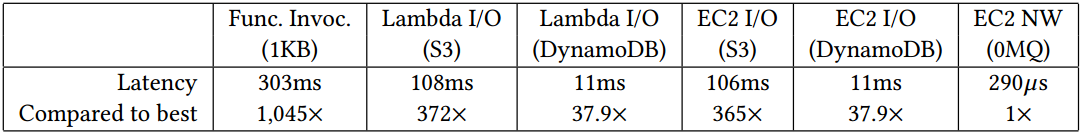
\includegraphics[width=0.7\linewidth]{figs/latency}
		\caption{将不同方式``通信''1KB的延时。为了刻画纯函数化的事件驱动通信,展示了在1KB的参数上调用一个空操作(no-op)Lambda函数,重复1000次取平均时延;接着展示了两个显式的从Python Lambda函数和EC2实例到S3和DynamoDB上的1KB I/Os (write+read)操作,重复5000次取平均时延;最后展示了直接用网络进行1KB的消息传递,使用Python和ZeroMQ消息库运行在两端的EC2实例上运行来测量出来的时延,重复10000次取平均时延。(\cite{hellerstein2018serverless}表1)}
		\label{figs:latency}
	\end{figure}
\end{enumerate}

所以针对目前基于FaaS的Serverless Computing的局限性和体现的问题,文章\cite{hellerstein2018serverless}放眼未来,提出了6点关键而明确的挑战:
\begin{enumerate}
	\item \textbf{流动的代码和数据放置}\ \ 弹性要求代码和数据在逻辑上分离,但是为了获得良好的性能,Serverless架构应该能够并且愿意物理的共享某些代码和数据。所以最好是将代码传动到数据,而不是将数据提取到代码的当前FaaS普遍做法。
	\item \textbf{异构硬件的支持}\ \ 允许开发人员通过规范将代码定位到特定硬件特征可能是有用的,以促进软硬件协同设计。但是对异构硬件的支持并不意味着就是提倡硬件和服务紧耦合。Serverless平台应该根据程序员提供的或从代码中提取的逻辑性能要求规范,对区分资源的代码分配做出动态的决策。然后可以将这些规范用于更一般的异构性感知来进行资源的时空复用\cite{tumanov2016tetrisched}。
	\item \textbf{长期运行,可寻址的虚拟代理}\ \ 因为FaaS中的函数不具有数据的亲和性,并且没有网络可寻址性,所以重复的请求无法充分利用先前的缓存数据。这样,最好能偶股提供一个长期运行住手在平台上的虚拟代理,而且这个代理是可寻址的。用它来指导函数在哪个具体的VM上运行,以在重复的请求中利用好缓存,来减少数据的传输。
	\item \textbf{无序编程模式}\ \ 如果要真正做到分布式计算时对资源的大小进行自动弹性的调整,更本质的是在编程的模式有所突破,这便是无序的,或者说异步的模式(不同于冯诺依曼体系结构)。
	\item \textbf{灵活编程模式和通用的中间表示层}\ \ 对每个语言来说,实现一整套相关优化是繁重的。所以就非常有必要提供一种用于云端的通用的中间表示层,任何高级语言都可以将代码编译成这个中间层,从而能够统一实现对上文提到的流动的代码和数据放置、异构硬件和无序编程模式这三个挑战的优化和支持。
	\item \textbf{安全性考虑}\ \ 颇为矛盾的是,如果上述的几个挑战在未来都能够得到很好的解决,就会使得Serverless的运维责任方(一般来说也是Serverless平台的供应商)更难以提供安全性的保障。例如允许代码流向共享数据会加剧与多租户机制相关的安全管理挑战以及恶意代码在客户之间利用侧信道攻击收集机密信息的可能性。但是好的一方面是,在安全性上的创新会给新的研究带来机遇——学术圈又有新的工作可做了。
\end{enumerate}

\cite{hellerstein2018serverless}的作者Hellerstein给我的印象确实是这般观点犀利的。我在2018年在加州大学伯克利分校访学的时候,非常凑巧地上过他给本科生教授的数据库系统的课程。

\subsection{Cloud Programming Simplified:
A Berkeley View on Serverless Computing}
文章\cite{jonas2019cloud}论述的套路类似,通过实例应用来暴露出当前Serverless computing平台的局限性,借此提出改进这些局限性的挑战。

这里选择了5个研究项目。1)ExCamera:旨在为向YouTube等网站上传视频的用户提供实时编码服务;2)MapReduce:大数据分析框架,也包括其开源实现的Hadoop和Spark\cite{jonas2019cloud};3)Numpywren:大规模的线性代数计算;4)Cirrus:机器学习训练;5)Serverless SQLite:数据库服务。因为它们本来都是基于传统Serverful云计算的应用,所以文章的研究团队尝试着使用cloud functions来将这些应用改写成serverless版本。而那些阻碍改造的难点就非常自然的凸显出来了。不难发现,除了最后一个Serverless数据库外,前四个项目改造为Serverless computing模式的动机都非常的类似。那就是在这些应用整个计算的过程中,对资源的需求量波动都很大。如:ExCamera的计算量取决于视频文件的大小,从几MB到几GB不等;MapReduce处理有些任务的数据集大小变化会非常明显;Numpywren这类的科学计算量波动;机器学习中有若干步骤,比如预处理、模型训练和超参调整,不同步骤需要的计算资源量也存在这显著的差别。所以如果使用固定数量的集群会造成计算的缓慢(机器数量太少)或者资源的浪费(机器数量太多)。利用serverless计算的弹性缩放扩容能力可以很好的平衡计算速度和资源利用率,同时还可以把科研人员,特别是没有体系结构只是背景的开发者从管理集群的繁琐任务中释放出来。最后的成本---性能结果为:ExCamera性能比VM实例提高了60倍,价格却便宜了6倍;MapReduce排序100TB数据仅比VM实例快了1\%,但多出了15\%的成本;Numpywren完成时间慢了3倍,不过CPU资源的消耗量低了1.26到2.5倍;Cirrus比VM实例快了3到5倍,但是开销也高出了7倍;Serverless SQLite如果仅用cloud functions的FaaS形式实现非常糟糕,因为这些函数独立运行,不能共享内存,而且也无法网络直接寻址,需要利用一些远程持久性存储,这会带来较大的延迟(这一点已在文章\cite{hellerstein2018serverless}的解读中反复出现)。所以数据库的一个合理的做法是依然保留为BaaS的形式。

从实际的用例选择与分析上不难发现,文章\cite{jonas2019cloud}比\cite{hellerstein2018serverless}要乐观很多,或者说要中立客观一些。文章\cite{hellerstein2018serverless}所选择的3个实例在传统的云计算无论是性能还是成本大获全胜,这样的分析不免就显得有些偏颇,而有失客观,有刻意迎合自身论证的嫌疑。事实上,Serverless computing后于传统的Serverful云计算提出,又在短时间内获得了大量的关注、讨论和应用,说明它肯定是有自己的过人之处与合理的地方。这在ExCamera的用例中,我们就能看的非常清楚,成本和性能全面提升。所以这种简单的应用就非常适合使用Serverless computing。除了Serverless数据库外,另外的3个用例在两个模式中各有千秋。Serverless方案要么性能高,但是成本也高;要么资源利用率高,但是性能低。只有数据库这种传统的分布式系统让Serverless模式颇为难堪。

接下来是文章\cite{jonas2019cloud}列举的这些应用切换到Serverless模式尴尬的局限之处,和\cite{hellerstein2018serverless}有重合之处,但是态度要温和很多。
\begin{enumerate}
	\item Serverless平台的无状态特性使得很难支持具有细粒度状态共享需求的应用程序,这主要是由云供应商提供的现有的存储服务所限制的。如AWS S3、Azure Blob Storage和Google云存储之类的对象存储服务都具有很高的可伸缩性,并且有廉价的存储成本;但是具有较高的访问成本和延时。而如键值数据库如AWS DynamoDB虽然需要长时间进行扩容,而且存储价格相对高昂,但是优势是访问延迟小。
	\item 接下来的两点在上文的\cite{hellerstein2018serverless}解析中也均有提到,反映了Serverless在分布式系统中的弱势。首先Serverless缺乏细粒度的协调机制;其次,Serverless在标准通信模式中性能表现的很差劲。在分布式系统中,广播、聚合和shuffle是非常常见的3种通信原语。这些操作也被经常用于机器学习训练和大数据分析所使用。图\ref{figs:pattern}展示了基于VM和Serverless函数的这3个通信模式的异同点。不难看出基于VM的方案需要远程发送的消息数量比基于Serverless cloud functions的方案大大减少了。这是因为在同一个VM实例上运行的若干任务可以共享数据广播的副本,或者在将部分结果发送到其他实例之间先执行本地聚合。但是因为应用程序无法控制cloud functions的位置(也即位于哪个VM中),就所以无法像VM一样利用好局部性,尤其是shuffle的复杂度大大提高了。
	\begin{figure}[!htbp]
		\centering
		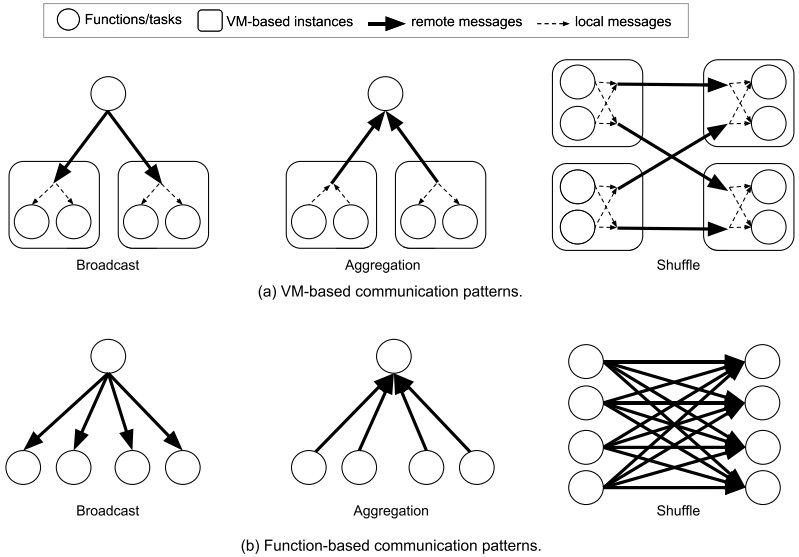
\includegraphics[width=0.6\linewidth]{figs/pattern}
		\caption{通信模式从左到右依次为广播、聚合、shuffle。(a)展示了VM实例上的运行情况;(b)展示了cloud functions实例上的运行情况。}
		\label{figs:pattern}
	\end{figure}
	\item 性能的不可预测性。正所谓成也萧何败萧何,函数运行环境有第三方管理大大简化了程序员的工作,但是也会带来性能的不确定性,比如分配到了不同的硬件资源。其中最突出的问题是冷启动,有三个影响因素:1)启动cloud functions所需要的时间;2)初始化函数的软件环境所需要的时间,如加载Python库;3)用户代码中特定应用程序的初始化。后两个因素往往占主要部分——启动一个cloud functions可能需要不到1秒,但加载所有应用程序库可能需要几十秒。简单的Serverless函数本身运行也不过最多几分钟到十几分钟罢了。
\end{enumerate}

同样的,文章\cite{jonas2019cloud}也提出了Serverless领域未来发展需要解决的挑战,系统地考察了五个领域:
\begin{enumerate}
	\item \textbf{抽象}\ \ 对资源的控制权重口难调,特别是硬件加速器的流行。目前的Serverless抽象阻碍了用户获得对加速器更多的控制权。所以需要提高抽象层次,可以让云供应商推断资源需求,而不是让开发人员执行它们。可以采用的方法有多种,如从静态代码分析以前的运行情况,接着动态重新编译,将代码重定向到其他体系结构。另外Serverless computing的低效的通信模式也是一直所诟病的,如MapReduce和numpywren用例所示。一个解决方案是云供应商公开一个API允许(可选)应用程序指定其计算图谱,从而实现更好的代码数据部署决策,最小化通信开销以提高性能。\cite{jonas2019cloud}的研究团队已经注意到许多通用的分布式框架(如MapReduce、Apache Spark和Apache Beam/Cloud Dataflow)、并行SQL引擎(如BigQuery、Azure Cosmos DB)以及编排架构(如Apache Airflow)其实已经在内部生成了这样的计算图谱。所以原则上,很方便的就能够做到Serverless平台的移植,并通过API向云供应商提供运行的计算图谱。
	\item \textbf{系统}\ \ 这一领域是旨在解决存储和冷启动问题。存储不仅要考虑延时、价格,容错也是必须考虑的。另外,存储还分为临时性存储和持久性存储。而面对冷启动,核心的思想在于尽可能缩减启动量以及提前缓存或者预取。
	\item \textbf{网络}\ \ 和抽象领域中的通信模式重合,最好的解决方案也是让应用程序提供一个计算图谱,使云供应商能偶定位cloud functions,以最小化通信开销。
	\item \textbf{安全}\ \ 这个之前的文章\cite{hellerstein2018serverless}中就有提到,但是并未给出具体的解决之道。Serverless computing重新划分了安全职责,将其中的大部分从云用户转移到了云供应商。然而,Serverless computing还必须解决应用分解后多租户资源共享所固有的风险。物理共享存储是在云平台内部引发硬件级别侧信道攻击和Rowhammer攻击的主要原因。此类攻击首先会寻找和攻击目标位于同一物理主机上的租户作为入侵对象。不过cloud functions的生命周期比较短,且调度存在随机性,会使攻击者难以找到和侵入对象。所以使用一种随机化的、能感知入侵的调度算法将会大大降低此类攻击发生的可能性。但是这样产生的物理隔离有可能会导致启动时间增加、资源利用率降低以及低效通信等问题再次涌现。另外,云函数需要细粒度的安全环境配置,包括获得私钥、存储对象等,并为cloud functions提供易表达的安全接口。值得警惕的是,cloud functions是一把双刃剑,它会通过通信泄露其访问模式和时间信息。而且云函数因为短暂且广泛地分布在整个云上,即便是进行了端到端加密,也有泄露的分解。二阶将Serverless应用分解为许多功能单一的小函数的趋势加剧了这种安全性风险。不幸的是,已有的方法如oblivious算法的开销往往很高。
	\item \textbf{体系结构}\ \ 说到底就是目前对异构硬件的支持不够,其中的观点和\cite{hellerstein2018serverless}类似。
\end{enumerate}

虽然两篇文章论述的套路相似,但是文作者Jonas对Serverless computing表现出来的态度却要乐观很多。他认为上述讨论的Serverless computing的局限性和挑战终将会被克服。困哪只是暂时的,Serverless computing会成为未来云计算的门面\cite{jonas2019cloud}。同时,他的研究团队更是盛赞Serverless computing的出现代表了类似于从汇编语言到高级语言的转变\cite{jonas2019cloud}。这个类比不无道理:高级语言将程序员从寄存器分配和内存管理的繁杂任务中解放出来,提高了逻辑的抽象层次,从而提高了程序员的编程效率;类似的,Serverless computing将程序员从云端的虚拟资源分配和服务器运维的复杂任务中解放出来,使得程序员更加集中精力于业务自身逻辑的应用开发,从而提高开发效率。
%TODO:一个有意思的哲学思辨
%TODO:Google和Azure提供的Severless相差不大。

\section{Amazon AWS Lambda深入---Firecracker(周盈坤)}\label{sec:Firecracker}
%TODO: 强调一下light-weight virtualization technologies
在章节\ref{sec:lambda}中,我们介绍了Lambda早期搭建在EC2虚拟机实例上的Linux容器的组织与管理。并在章节\ref{sec:lambda}的最后提及由于其明显的局限性,Amazon在2018年re:invent大会上宣布开源了一个新的项目工程:Firecracker微虚机(microVM),并已经应用在了Lambda服务之中。

\subsection{概念梳理}
Firecracker与先前的Linux容器方案是有区别的,但是这种区别在认知中容易混淆。这里我们不妨先来厘清楚各种技术之间错综复杂的概念之间的关系。

首先,现在普遍采用的隔离(isolation)技术有三种,分别是\cite{agache2020firecracker}:
\begin{figure}[!htbp]
	\centering
	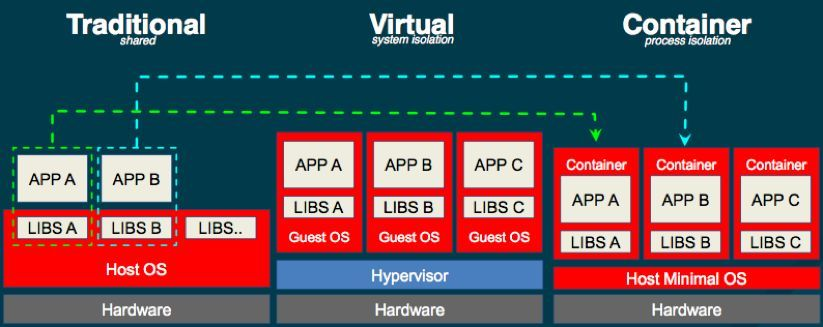
\includegraphics[width=0.8\linewidth]{figs/isolation}
	\caption{从左到右依次为传统的应用进程共享内核结构(无法隔离)、虚拟化技术(应用运行在虚拟机上VM \& GuestOS,提供系统级别隔离)、容器技术(提供进程级别隔离)}
	\label{figs:isolation}
\end{figure}
\begin{enumerate}
	\item Linux容器,见图\ref{figs:isolation}最右子图;应用运行在容器中,不同的容器按照应用需求配置有不同的库;若干个容器运行在主操作系统内核上。LXC和Docker属于此类。另外,Google为了进一步解决容器的安全性和兼容性的的tradeoff,推出的gVisor也是容器中的一个具体实现。
	\item 虚拟化,见图\ref{figs:isolation}中间子图;应用程序运行在VM中,不同VM按照应用需求配置有不同的库;VM可以看做是Guest OS运行在Hypervisor层上。KVM、QEMU和Unikernel(为了解决冷启动高时间开销等问题)属于此类。另外,本章的主角Firecracker采用的正是此类方案。Firecracker基于KVM,但用更安全的编程语言Rust以及更少的代码(more code$ = $more bug)来替换QEMU。值得一提的是Firecracker包含大约5万行Rust代码,仅是QEMU代码量的4\%.
	\item 语言专用隔离(Language-Specific Isolation)。这一类隔离技术并未在图\ref{figs:isolation}中体现,但是读者一定不会陌生,因为Java虚拟机(JVM)就属于此类。
\end{enumerate}

光有隔离还不够,文章\cite{hellerstein2018serverless,jonas2019cloud}无一不在强调云平台上安全性的重要。为此我们可以在上述的隔离方案中嵌入沙盒(sandbox)机制来增强安全性,如图\ref{figs:sandbox}所示。沙盒对于\ref{figs:sandbox}(a)的Linux容器方案几乎是必选项,因为容器的安全隔离性不够强,需要沙盒加固;而对于\ref{figs:sandbox}(b)的虚拟化技术就是可选项了,因为VMM会内置安全隔离性。
\begin{figure}[!htbp]
	\centering
	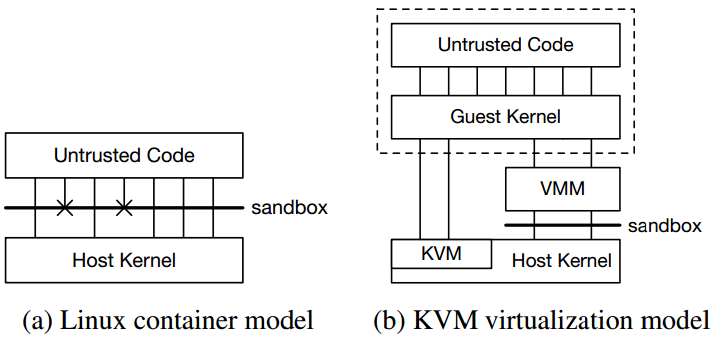
\includegraphics[width=0.5\linewidth]{figs/sandbox}
	\caption{(a) Linux容器的安全模型,直接依赖于内核沙盒的防御攻击能力;(b) KVM虚拟化的安全模型,依赖于Virtual Machine Monitor(VMM)的安全性,可配上沙盒来加固。(\cite{agache2020firecracker}图1)}
	\label{figs:sandbox}
\end{figure}
有了这些基础的背景知识,这里再次强调几点。首先,容器并不是一种虚拟化技术,而是一种进程隔离技术,从内核空间、资源和安全等方面对进程做隔离。其次,Firecracker基于虚拟化技术,因此不属于Linux容器的类别,所以和Google推出的gVisor有着本质的不同。最后,Firecracker不是一种新型的虚拟化技术,依然依赖Intel VT-x,只不过它做的比QEMU精简很多,目的就是完全取代QEMU。那么为什么要取代QEMU呢?原因有很多,例如:QEMU庞大的代码体积,其中很大一部分是对基本上用不到的传统设备、总线、机器模型的模拟。虽然能够对各种硬件协议做到真实模拟,一般来讲确实多多益善,但是近年来因为庞大的代码量而高发的漏洞数量,以及针对Serverless computing这样的场景,需要业务启动快、密度高、可快速自动缩扩容,就迫切需要像Firecracker这样提供更为敏捷的运行环境。另外,我们这里不提及Firecracker和Kata Container(由Intel、Hyper.sh和OpenStack主导)的差异。回到主角Firecracker的讨论。

\subsection{Firecracker implementation}
Firecracker像QEMU一样负责创建和管理微虚机。它提高了资源的利用率和计算效率,而且内存开销极低,使得在一台物理服务器上可以常见数千个微虚机。相比之间的Linux容器方案,简单陈列一下其好处有:利用CPU硬件虚拟化实现了用户之间的强隔离性;简化但增强了安全模型;简化了Lambda编程模型;提高了资源利用率;缩短了函数的启动时间。不像Kubernetes,Firecracker就是专门针对Serverless场景设计的,非常适合运行暂时性(transient and short-lived)进程。因为Firecracker是开源的,其网址为\url{https://firecracker-microvm.github.io/},所以有大量公开的信息和设计文档文章可供查阅,还可以直接阅读\href{https://github.com/firecracker-microvm/firecracker}{Github}上的源码。

结合公开的资料,首先我们能够分析出大致几点Firecracker的设计思路与原则。1)内置安全性,支持多租户工作负载的同时做到计算安全性屏障不会被用户有意或者无意的禁用;用户工作负载被认为既神圣不可侵犯的,但又是邪恶的,需要时刻提防。2)轻量虚拟化,重视短暂运行和无状态的工作负载,而非长时间运行和共享状态的工作负载;Firecracker的硬件资源开销是明确且有保障的。3)函数极简,不会构造AWS任务没有明确要求的函数,且每个函数代表的任务功能单一。4)资源的分时复用,Firecracker向用户开放的所有硬件计算资源都可以高效安全地复用。下面我们接着来看Firecracker VMM的特征和体系结构。图\ref{figs:Firecracker}展示的就是Firecracker一个比较完整的体系结构图景。其中,图\ref{figs:host}展示了一个在主机(host)上运行$ n $个Firecracker微虚机的例子:Firecracker运行在Linux的guest OS上(图中显示为Guest的绿色方框);这些guest OS运行在4.14或者更高版本的Linux主机上;蓝色方框和线条是模拟的网络设备;黄色方框和线条是模拟的块存储设备。图\ref{figs:internal}更进一步展示了Firecracker微虚机内部的结构:每个Firecracker进程封装有且仅有一个微虚机。进程里一共运行3种线程:API、VMM和vCPU。
\begin{enumerate}
	\item API线程负责Firecracker的API服务和相关的控制面板,以Unix domain socket的方式向主机提供了一个RESTful API格式的API接口端点。通过这个端点可以对微虚机进行管理和控制,包括:规格配置(如vCPU的个数,用户内存大小)、网络配置(添加网卡)、存储配置(添加虚拟盘,一种基于文件的块设备)、QoS(通过带宽限制和IOPS限制进行流控)、日志配置、启动配置(内核及其参数,根文件系统)、关闭微虚机。
	\item VMM线程向Guest OS暴露出了机器模型、最小化的老式设备模型、微虚机元数据服务(microVM metadata service, MMDS)和VirtIO虚拟网络设备和块设备(用以提供给Guest网络和存储访问服务),并配有I/O速率限制(支持用户按照自己的需求定义灵活的带宽和突发传送的限额)。VMM采用单线程时间驱动模型,对各种I/O请求进行服务。
	\item 除此之外,有一个或多个vCPU线程(每个guest CPU core各一个);它们通过KVM被创造出来,并且运行在\texttt{KVM\_RUN}主循环中;它们在设备模型中执行同步I/O和内存映射I/O操作。
\end{enumerate}
注意到图\ref{figs:internal}中特意标出了两个边界。内围的浅红色边界为Virtualization Barrier,利用虚拟化技术提供Customer Zone一个安全隔离的环境。外围的深红色的边界为Jailer Barrier,作为第二道防线,负责利用Linux提供的seccomp、cgroup、chroot、net/pid/user namespaces来创造沙盒环境;接着在其创造的沙盒环境中启动Firecracker VMM;最后,Firecracker VMM利用KVM创建含有设备模型等(见上文第2点)的极度精简微虚机(Firecracker Zone)。

Firecracker的开发者与开源社区有着积极的互动。而从这篇报告完成的时间2020年5月底,在Firecracker主页上,我们已经惊喜的发现:Firecracker已经和Kata Containers、Weave FireKube集成在了一起,通过firecracker-containerd实现与容器的对接。图\ref{figs:fire}展示了Firecracker VMM的整体架构。集成了上文所述的图\ref{figs:host}\ref{figs:internal}中的要素,也集成了容器的工作负载。这三幅子图中,虽然一些表述不同,但是含义是一致的,如\ref{figs:host}中的Guest(绿色方框)、\ref{figs:internal}中的Customer Zone(红色方框)、\ref{figs:fire}中的Guest OS \& Container workload(灰色方框)表示的是同一个意思。而且如果把\ref{figs:internal}由Jailer Barrier围住的方框倒过来,和图\ref{figs:fire}的右边结构(包括内外围的两个Barriers)就几乎是一模一样的。另外,图\ref{figs:fire}中左边的结构画的非常的形象——和店面中出租的共享手机充电插槽设备神似。Firecracker的底座Host Kernel Space上面上可以插上千个多租户的微虚机,而且各个微机的规模大小是可以参差不齐的,代表了工作负载量。
\begin{figure}[H]
	\begin{subfigure}[a]{0.49\linewidth}
		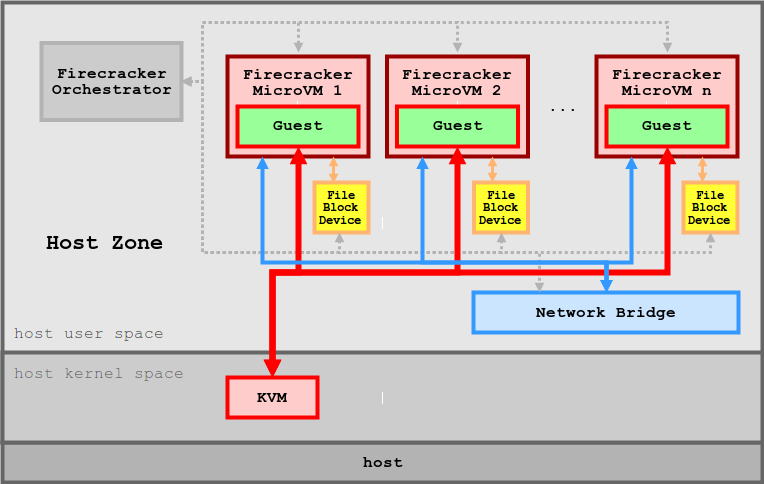
\includegraphics[width=\linewidth,height=0.27\textheight]{figs/firecracker_host_integration}
		\caption{}
		\label{figs:host}
	\end{subfigure}
	\begin{subfigure}[a]{0.49\linewidth}
		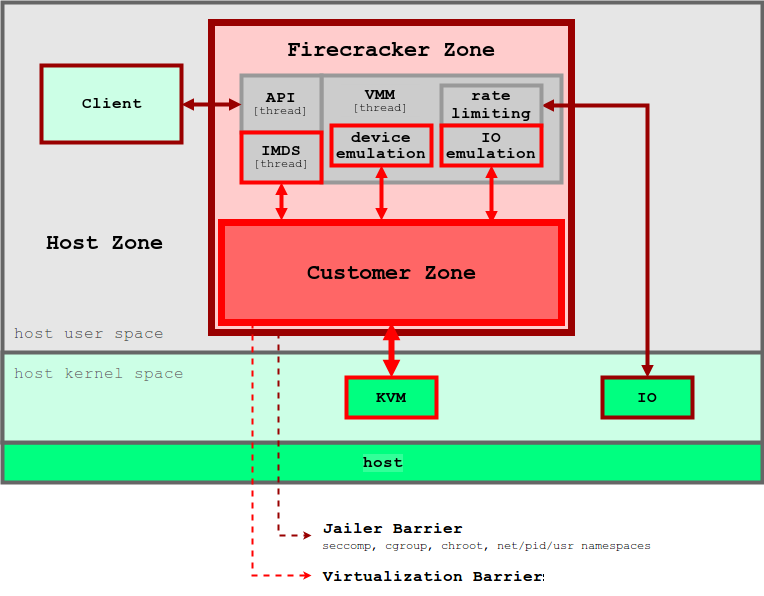
\includegraphics[width=\linewidth]{figs/firecracker_threat_containment}
		\caption{}
		\label{figs:internal}
	\end{subfigure}
	\begin{subfigure}[b]{\linewidth}
		\centering
		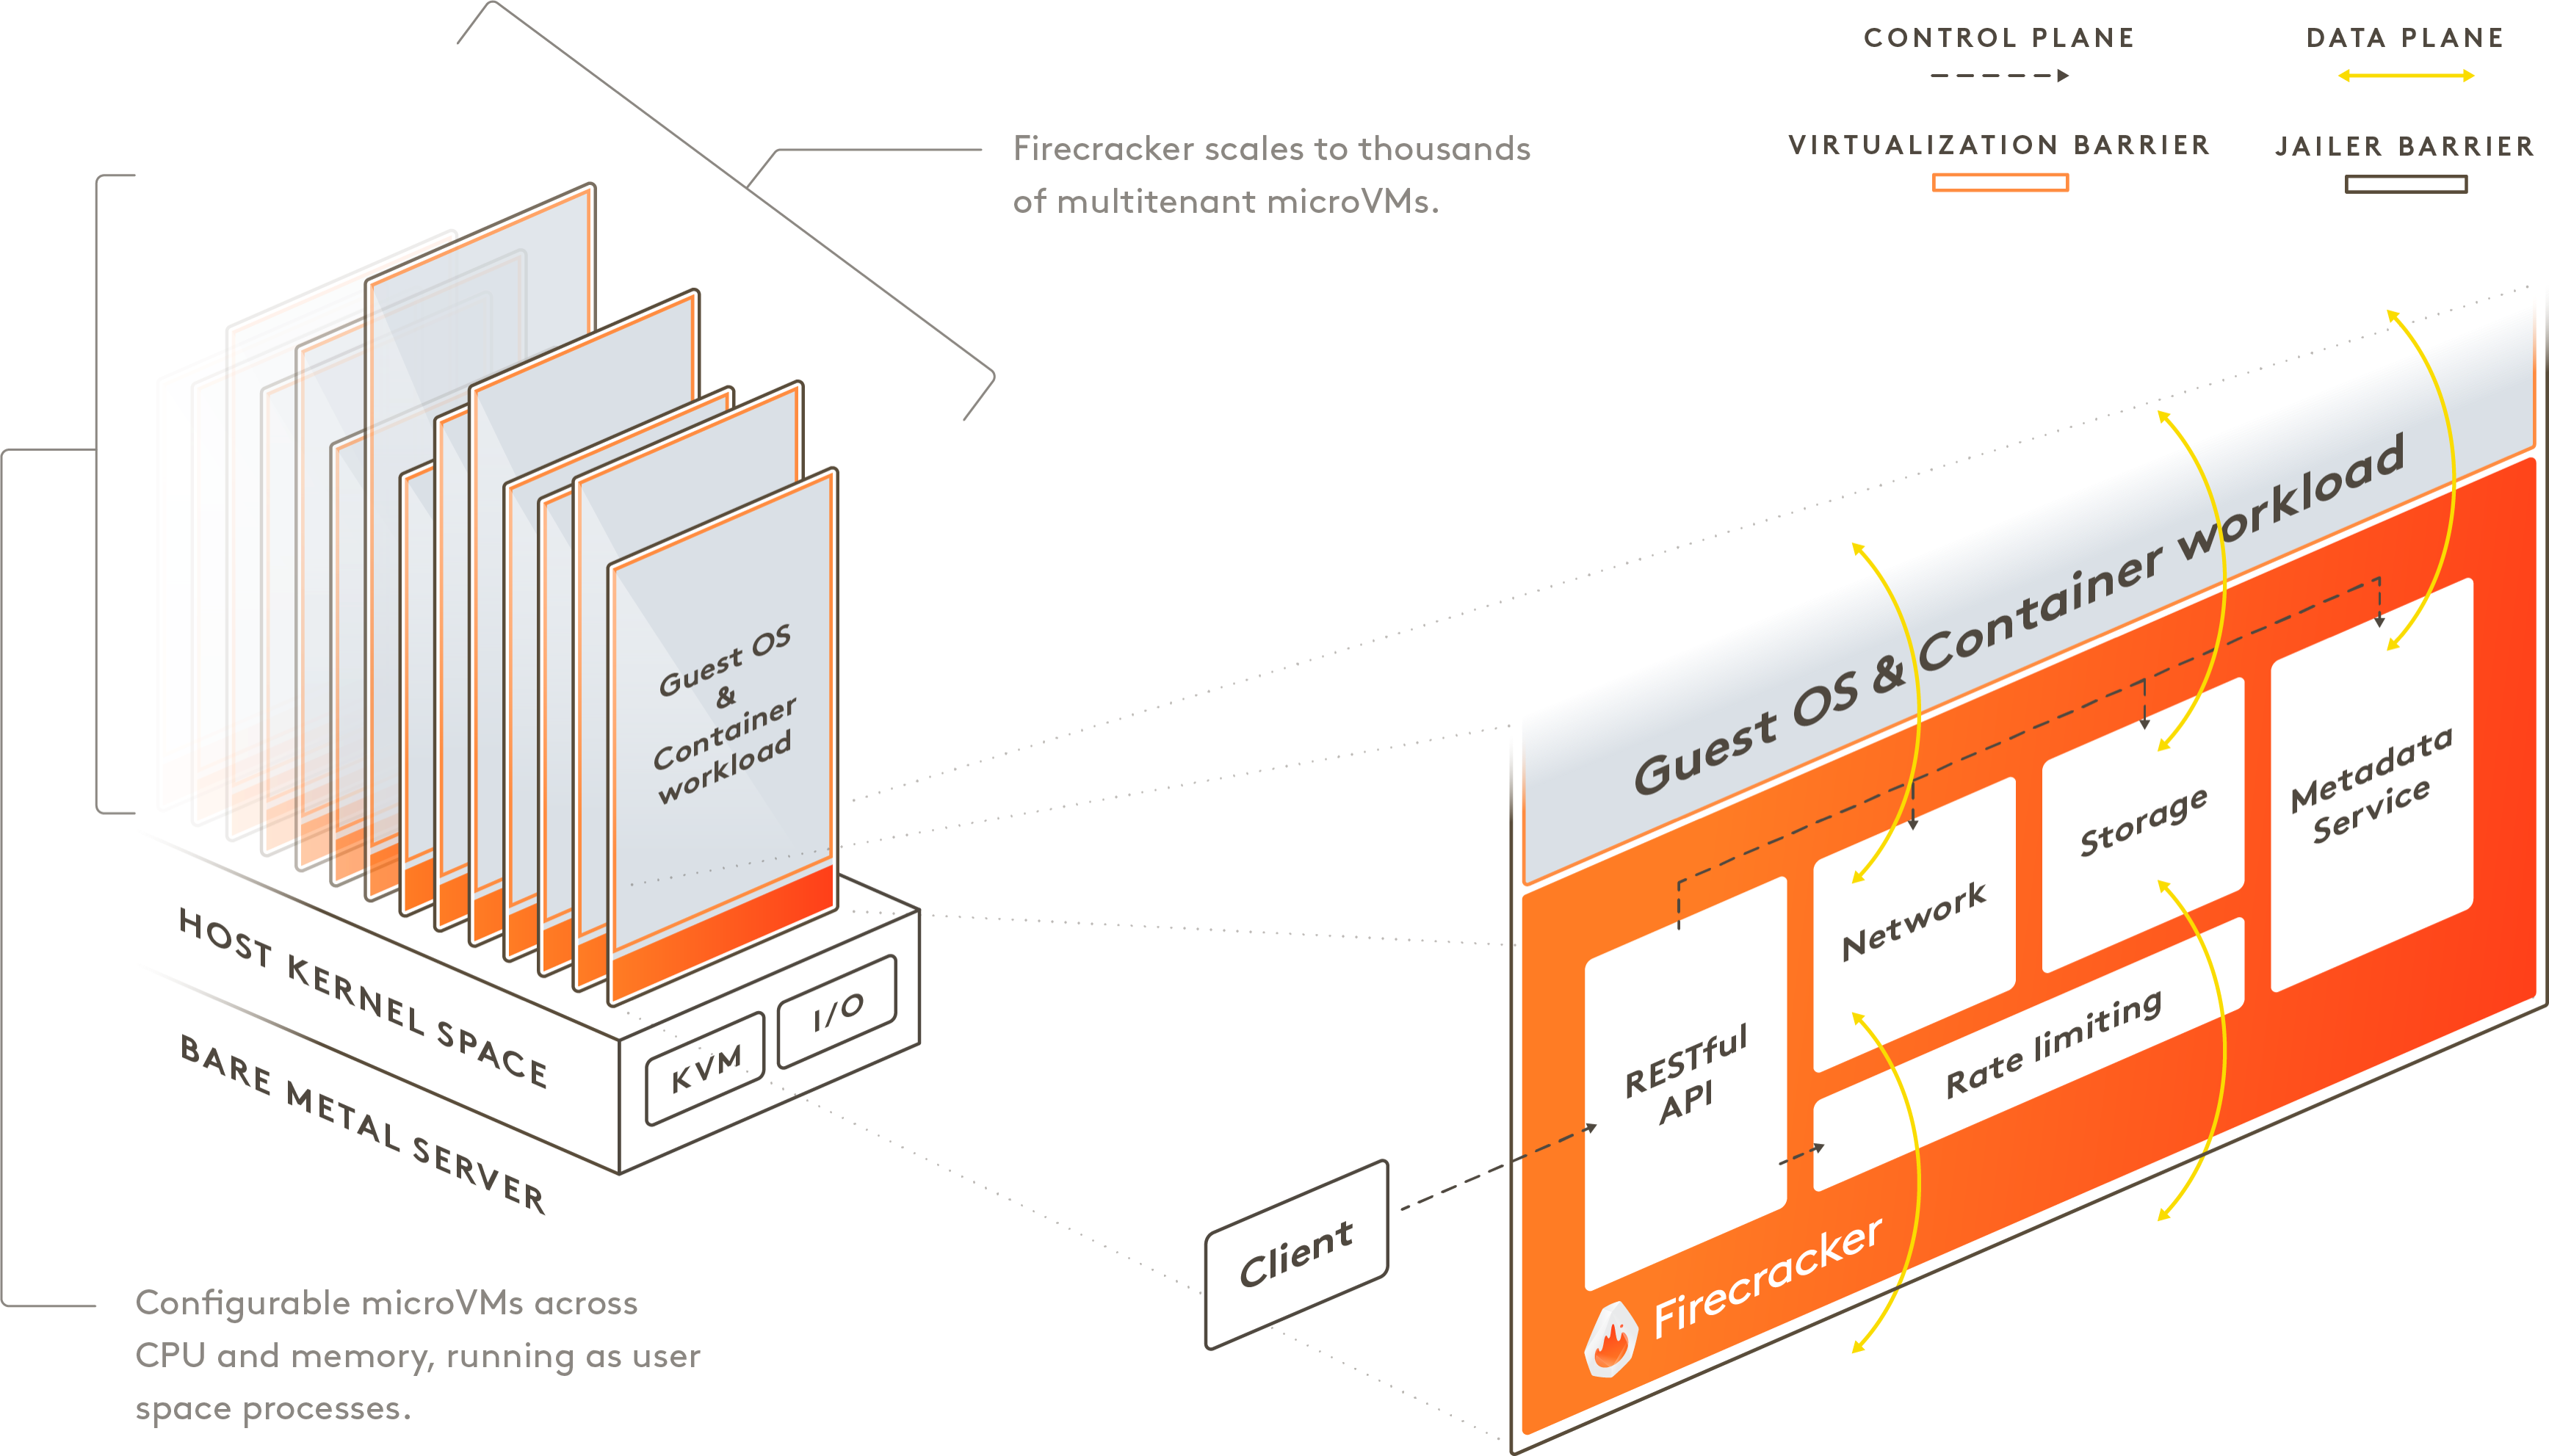
\includegraphics[width=0.8\linewidth]{figs/firecracker}
		\caption{}
		\label{figs:fire}
	\end{subfigure}
	\caption{(a) Host上运行多个Firecracker微虚机\cite{firecracker}。(b) Firecracker微虚机的内部结构\cite{firecracker}。(c) Firecracker VMM的整体架构\cite{fire}。}
	\label{figs:Firecracker}
\end{figure}

